% ===== 04-linear-regression =====
\section*{Linear Regression}

\subsection*{Motivation}
\begin{itemize}
  \item Self-driving car: input $\mathbf{x}$ = image of the road, output = steering direction.
  \item This is \textbf{supervised learning}: we get labeled pairs $(\mathbf{x}, t)$.
\end{itemize}

\subsection*{Running Example: House Prices}
Start by collecting a dataset of houses and their prices:

\begin{center}
\begin{tabular}{cc}
\toprule
Size (ft$^2$) & Price (\$1000s) \\
\midrule
2104 & 400 \\
1416 & 232 \\
1534 & 315 \\
852  & 178 \\
\vdots & \vdots \\
\bottomrule
\end{tabular}
\end{center}

Or plot size vs.\ price and fit a straight line through the points.

{\centering
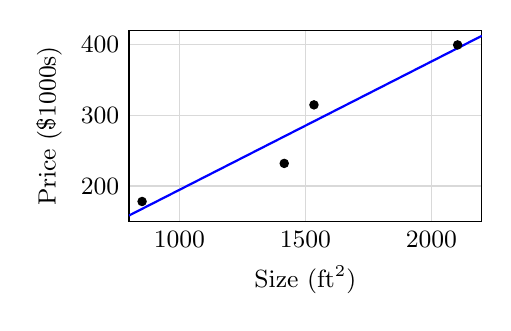
\begin{tikzpicture}
\begin{axis}[
    width=0.5\linewidth, height=4cm,
    xmin=800, xmax=2200, ymin=150, ymax=420,
    enlargelimits=false,
    grid=major, grid style={gray!30},
    major tick length=0pt,
    xlabel={Size (ft$^2$)}, ylabel={Price (\$1000s)},
    tick label style={font=\small}, label style={font=\small},
    xticklabel style={/pgf/number format/1000 sep={}}
]
\addplot[only marks, mark=*, mark size=1.5pt] coordinates {
    (2104,400) (1416,232) (1534,315) (852,178)
};
\addplot[thick, blue, domain=800:2200, samples=2] {12.5 + 0.182*x};
\end{axis}
\end{tikzpicture}
\par}

\subsection*{The Supervised Learning Pipeline}
\[
\text{Training set } \mathcal{D} \;\longrightarrow\; \text{Learning algorithm} \;\longrightarrow\; \text{Hypothesis } y(\mathbf{x}, \mathbf{w})
\]
\begin{itemize}
  \item The learning algorithm takes the training set and outputs a function (the \textbf{hypothesis}).
  \item The hypothesis takes a house we have not seen yet and outputs an estimated price.
\end{itemize}

\subsection*{Representing the Hypothesis}
One feature ($x_1$ = size):
\[
y(\mathbf{x}, \mathbf{w}) = w_0 + w_1 x_1
\]

Two features: add number of bedrooms.

\begin{center}
\begin{tabular}{ccc}
\toprule
Size $x_1$ & \# Bedrooms $x_2$ & Price $t$ \\
\midrule
2104 & 3 & 400 \\
1416 & 2 & 232 \\
1534 & 3 & 315 \\
852  & 2 & 178 \\
\bottomrule
\end{tabular}
\end{center}

\[
y(\mathbf{x}, \mathbf{w}) = w_0 + w_1 x_1 + w_2 x_2
\]

\textbf{Dummy feature trick:} define $x_0 = 1$ always, so the bias $w_0$ has a feature to multiply and fits inside one dot product $\mathbf{w}^\top\mathbf{x}$. Then
\[
y(\mathbf{x}, \mathbf{w}) = \sum_{d=0}^{D} w_d x_d = \mathbf{w}^\top \mathbf{x},
\qquad
\mathbf{x} = \begin{bmatrix} 1 \\ x_1 \\ x_2 \end{bmatrix},\;
\mathbf{w} = \begin{bmatrix} w_0 \\ w_1 \\ w_2 \end{bmatrix}
\]
Example: $\mathbf{w} = [50,\, 0.1,\, 20]^\top$, house $(2104, 3)$:
$\mathbf{w}^\top\mathbf{x} = 50(1) + 0.1(2104) + 20(3) = 320.4$.

\subsection*{The Loss (Least Squares / OLS)}
\[
E(\mathbf{w}) = \frac{1}{2}\sum_{n=1}^{N} \Big( \underbrace{y(\mathbf{x}_n, \mathbf{w})}_{\text{prediction}} - \underbrace{t_n}_{\text{target}} \Big)^2
\]
\begin{itemize}
  \item Squared difference between prediction and true value, summed over all $N$ examples.
  \item The $\tfrac12$ only cancels the 2 when differentiating; it does not change the minimizer.
\end{itemize}

We want the weights that minimize the loss, $\mathbf{w}^* =  \arg\min_{\mathbf{w}} E(\mathbf{w})$. We can find them using \textbf{gradient descent}.
